%!TEX root = ../main.tex

\graphicspath{{./figures/chapter2/}}


\chapter{Single RNA Detection}
\label{ch:chapter2}

\minitoc
\newpage

In this chapter we review different techniques for spot detection.
Even though the problem is not new, and has been largely addressed by different scientific communities, none of the suggested methods really meet the requirements of a high content screening analysis with \ac{FISH} experiments.

The second part of this chapter therefore describe our own implementation in \mbox{\emph{bigfish.detection}}.
We try to answer specific limitations of existing solutions, especially the possibility to scale the detection.
As an example, we also add a code snippet at the end of each step.

Finally we evaluate the robustness and the accuracy of our implementation by simulating spots under different noise conditions.

\section{Spot detection as a signal processing problem}
\label{sec:detection_introduction}

We first describe inputs and outputs we can expect when we perform spot detection.
Then we review some solutions proposed in the literature, in bio-informatics, but more generally in computer vision.
Lastly, we briefly discuss recent methods based on a deep-learning framework.

\begin{figure}[h]
    \centering
    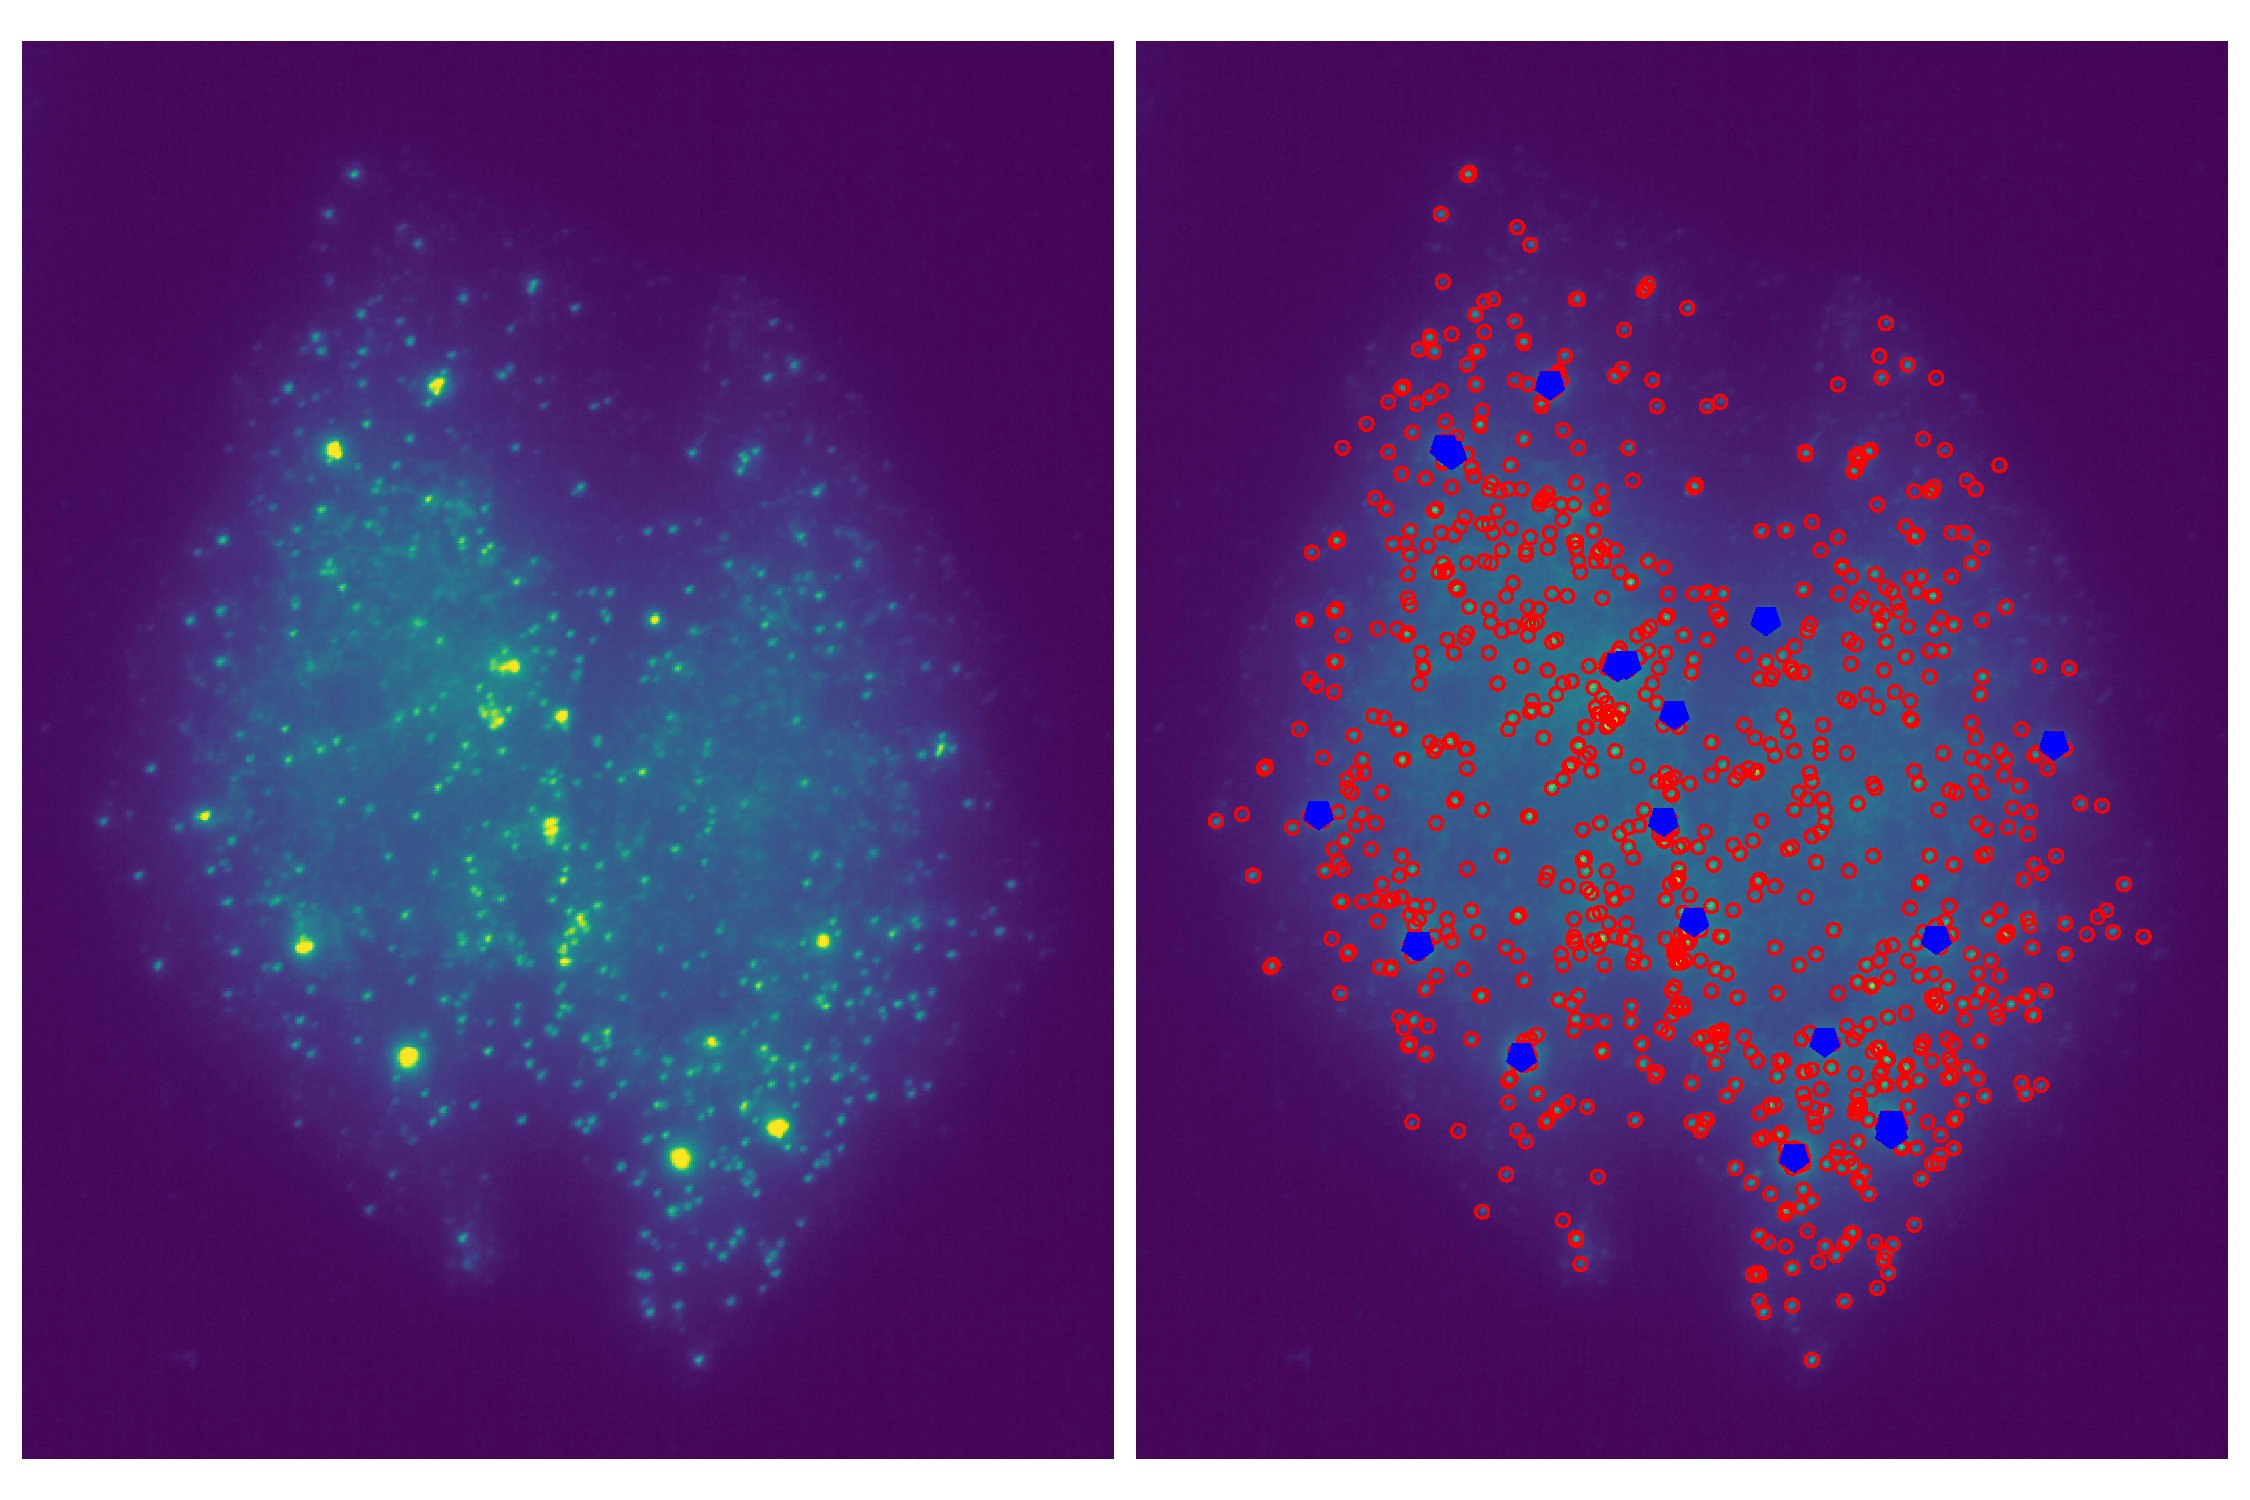
\includegraphics[width=1\textwidth]{figures/chapter2/cluster_detection_results}
	\caption{Detection results.
	(\textit{Left}) Original smFISH image.
	(\textit{Right}) Spots in \textit{red} and clusters in \textit{blue}, detected with \emph{bigfish.detection}}
    \label{fig:detection_results}
\end{figure}

\subsection{Extract spot coordinates from an image}
\label{subsec:detection}

Aim of spot detection is to extract a array of spatial coordinates from an image with identifiable point sources.
This task is performed in two or three dimensions, depending of the input image.

Detecting an object as small as a \ac{RNA} molecule implies some constraints.
The optical system does not capture the original light signal emitted by the fluorescence probes, but its convolution with a \ac{PSF}.
However, for the rest of the chapter, we simply assume the resulting spot signal can be approximate by a gaussian signal.
Such simplification is reasonable for a detection with a pixel accuracy, with our noise level.
In addition, as we can observe in Figure~\ref{fig:detection_results}, a \ac{smFISH} image often present a background fluorescence that doesn't identify with a \ac{RNA}.
The noise can be highly heterogeneous and vary between images and even cells.\\

\noindent
We can observe two types of noise:
\begin{itemize}
	\setlength\itemsep{0.1em}
	\item At the \ac{FoV} level, the noise from the optical setup itself and the experimental conditions.
	\item At the cellular level, the difference in the autofluorescence of the observed samples.
\end{itemize}

In the context of a high content screening study, numerous images are acquired, with various biological samples or conditions.
This leads to potentially heterogeneous pixel intensity and spot distribution across different images.
Spot detection can be really challenging.
It thus requires a robust approach to tackle this problem and extract accurate coordinates.

\subsection{Related work}
\label{subsec:detection_related_work}

\subsubsection{Threshold based methods}

Spot detection, especially with fluorescent images, has been addressed by the scientific community through different approaches.
Yet, some similitudes can be observed and difficulties remained.

\paragraph{Noise, signal and threshold}

A general review~\cite{smal_quantitative_2010} defines most detection frameworks with three steps: noise reduction, signal enhancement and signal thresholding.
As for the noise reduction, they detailed in particular Gaussian smoothing technique, a method we exploit ourselves in the next section, and wavelet-based filtering.
The later consists in applying a wavelet transform to obtain a sparse representation of the image, modifying the wavelet coefficients and transforming back the image.
For this inverse transformation, we only keep the largest wavelet coefficients that correspond to structural elements in the image.
Signal enhancement is then the most critical step.
Seven unsupervised methods are compared, including techniques like top-hat filter, \ac{LoG} filter or h-dome transformation.
This transformation is a reconstruction by dilation $\mathcal{B}(x, y)$ of the original image $f(x, y)$, from an image $f(x, y) - h$, with $h$ a positive constant.
As a result, we can decompose the original image such that $f(x, y) = \mathcal{H}(x, y) + \mathcal{B}(x, y)$, with $\mathcal{H}(x, y)$ the h-dome image with the remaining spots and local intensity peaks.
It can be interpreted as a local background subtraction technique that cut-off ''intensities of height h from the top, around local intensity maxima''.
Unlike previous mentioned filters, it does not involve any shape or size parameter, but a height parameter $h$.
Based on their experiment, authors favor this technique when a good detection performance is needed.
However, when image quality is great and the \ac{SNR} high enough, all the detection methods tested in~\cite{smal_quantitative_2010} perform well.
Finally, the signal thresholding discriminates the relevant spots from the noise, depending of the detection method applied.
Supervised techniques are also discussed and evaluated like the training of an ADABOOST model~\cite{FREUND1997119} with Haar-like features.
These methods appear to be accurate, even with low \ac{SNR} images, but require annotated data and a training stage.

Review from~\cite{ruusuvuori_evaluation_2010} completes the analysis with additional algorithms: kernel-based methods, Otsu thresholding~\cite{Otsu_1979} or source extraction~\cite{bertin_sextractor_1996}.
The later is mainly applied in astronomy.
It thresholds an image where the background has been estimated then subtracted, before deblending adjacent spots.

\paragraph{Implementations}

Several detection algorithms are already implemented and easily available in popular Python packages like \emph{scikit-image}~\cite{walt_scikit-image_2014} or \emph{astropy}~\cite{astropy_2018}.
Astropy community developed an affiliated package \emph{photutils}~\cite{larry_bradley_2020_4044744} with helpful functions for photometry of astronomical sources like \ac{PSF} matching or source detection.
Additional software focused on fluorescent image analysis, but not always in Python.
They propose their own spot detection pipeline like Icy~\cite{de_chaumont_icy_2012} (with a wavelet-based method) or Trackmate~\cite{ershov_trackmate_2022} (with a blob detection method).
The recent Python library \emph{starfish}~\cite{perkel_starfish_2019} wraps existing \emph{scikit-image} functions and the first FISH-quant version~\cite{mueller_fish-quant_2013} includes a blob detection pipeline with a \ac{LoG} filter.
This last pipeline is the one we implemented and improved for \emph{bigfish.detection}.

More recently RS-FISH~\cite{bahry_rs-fish_2021} was released specifically for 3D spot detection with \ac{FISH} images.
Developed in Java and exploiting radial symmetry, it presents a great subpixel accuracy, a fast runtime computation and robustness against anisotropic spot signal.
After a \ac{DoG} filtering, we threshold the image to generate potential spot localizations.
We then extract image gradients around each spot and correct them for anisotropy.
Besides possible outliers that are filtered out, gradients should point toward a common center: the spot localization.
In addition to their code, authors released a plugin for Fiji software~\cite{schindelin_fiji_2012}.
Such \ac{GUI}, is not new: Icy, Trackmate and FISH-quant also have one.
Like these alternatives, it allows the user to manually tune parameters and find the optimal setup for his application.

This last point is a major limitation for us.
The need for parameter tuning is a critical bottleneck for scaling detection.
When we apply an algorithm to thousands of images, with noise and intensity heterogeneity, most parameters need to be set once (or automatically) and not recalibrated between images.
In particular most of the presented methods require a threshold or a size parameter at some point.

% add a detailed description of top-hat filter
% add reference top-hat filter and h-dome transformation
% add exemples from smFISH, seqFISH+ and MERFISH applications

\subsubsection{Learning to spot}

Scaling of spot detection has been addressed by recent deep learning methods.
They intend to prevent parameter tuning on a cell-by-cell or image-by-image basis at the cost of a learning stage.

A first study~\cite{bouilhol_deepspot_2022} proposes to preprocess images to make spot intensity homogeneous.
They trained DeepSpot, a convolutional network, to enhance spot signal to the same intensity.
The network has two main components: a \ac{CASO} module followed by a customized ResNet~\cite{He_2016}.
\ac{CASO} mixes standard convolution blocks with strided and atrous (or dilated) convolutions~\cite{Hamaguchi_2018}.
Small objects like spots do not contain enough semantic information to be captured.
Standard convolution blocks (with max pooling) are great to learn semantic information, but at the expense of lower intensity spots and a potential spatial information loss.
One the one hand, replacing the pooling layer with strided convolution compensates the lower intensity.
On the other, the use of atrous convolution increases receptive field and thus improves context information with a minimal spatial information loss.

Another model, DeepBlink~\cite{eichenberger_deepblink_2021}, is based on a U-Net architecture~\cite{Ronneberger_2015} and directly detects spots.
The U-Net component extracts intermediate features.
Then it maps the original image into \emph{grid-cells} (small bounding-boxes) for which model predicts the probability of a spot localization and the potential 2D coordinates.
Size of the \emph{grid-cell} is critical.
With a small size, too many cells might be empty, resulting in an imbalanced dataset for the classification head of the model.
On the opposite, with a larger size, one cell could contain multiple spots (for only one prediction per \emph{grid-cell}).
This process is directly inspired by the detection model YOLO~\cite{Redmon_2016_CVPR}.

\section{Scaling \ac{mRNA} detection}
\label{sec:method}

We now describe at depth the algorithms currently implemented in \emph{bigfish.detection}.

\subsection{Spot detection}
\label{subsec:spot_detection}

The method we use is directly adapted from the original version of FISH-quant~\cite{mueller_fish-quant_2013} and the blob detection algorithms~\cite{walt_scikit-image_2014}.
Detection is performed in 2D or 3D. Image is filtered in order to increase its \ac{SNR}, then each spot is defined as a local maximum above a specific threshold.

\subsubsection{Filtering}

We apply a \ac{LoG} filter (one Gaussian filter followed by a Laplacian one).
It's a two-step algorithm that enhances the spot signals.
The first Gaussian filter smooths the image and removed the high frequency noise.
The second Laplacian filter approximates the second derivative of the image.
We apply this operator at a single scale because we assume a unique size for the spots.
By default, the size of the Gaussian kernel is set to match the expected size of the spot.
The latter is assumed to be known for a given experiment and should not prevent the user to scale the detection.
If we consider a 2D image $f(x,y)$, the \ac{LoG} filter consists in computing the second derivative of the smoothed image $L(x, y, \sigma^2)$:

\begin{equation}
	{\displaystyle \nabla^{2}L(x, y, \sigma^2) = \frac{\partial^{2}L(x, y, \sigma^2)}{\partial x^2} + \frac{\partial^{2}L(x, y, \sigma^2)}{\partial y^2}}
\end{equation}

\noindent
with $L(x, y, \sigma^2)$ the convolve image:

\begin{equation}
	{\displaystyle L(x, y, \sigma^2) = g(x, y, \sigma^2) * f(x, y)}
\end{equation}

\noindent
and $g(x, y, \sigma^2)$ the Gaussian kernel with a scale $\sigma^2$:

\begin{equation}
	{\displaystyle g(x, y, \sigma^2) = \frac{1}{2\pi \sigma^2} e^{-{\frac{x^{2} + y^{2}}{2\sigma^2}}}}
\end{equation}

An alternative filter is the \ac{DoG} filter.
We estimate the background of the image with a large Gaussian kernel, then we subtract it from the original image or one smoothed with a narrower Gaussian kernel.
It is a fast approximation of the \ac{LoG} filter.
As illustrated in Figure~\ref{fig:filters_detection}, both methods aim to remove the background noise and enhance the spot signal.

% reference LoG and DoG

\begin{figure}[h]
    \centering
    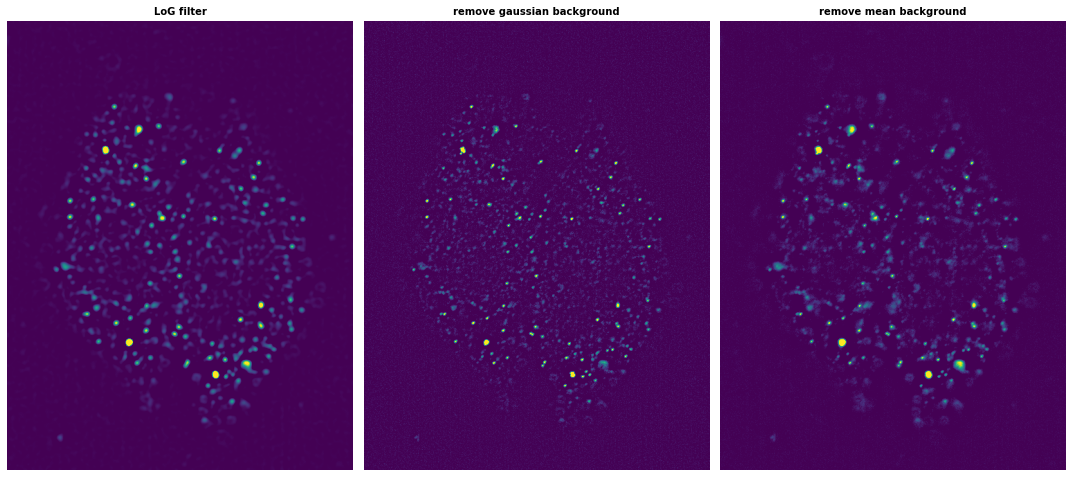
\includegraphics[width=1\textwidth]{figures/chapter2/filter_background}
    \caption{Filtered images with LoG filter (\textit{Left}) and DoG filter (\textit{Right})}
    \label{fig:filters_detection}
\end{figure}

\subsubsection{Peak detection}

A Local Maximum detection algorithm follows the filtering.
We apply a maximum filter on the \ac{LoG}-filtered image and compare the result to the original one.
A pixel with the same value in the original and filtered images is defined as a local maximum.
If, by chance, a spot has several identical pixels at its peak, we only keep one to define the spot coordinate.

% reference local maximum algorithm

\subsubsection{Thresholding}

At this stage, actual spots and noisy fluorescent blobs (autofluorescence, of-site binding of oligos, etc.) are both detected.
From all previously detected local peaks, we only keep those above a specific threshold.
A first limitation of spot detection algorithm appears with the choice of this threshold.
If it is manually set, it might be difficult to scale the method to a large experiment as the fluorescence can be quite heterogeneous between images.
Thus, we use a heuristic technique to set a threshold per image in a automated way.

\begin{wrapfigure}{L}{0.35\textwidth}
	\begin{center}
		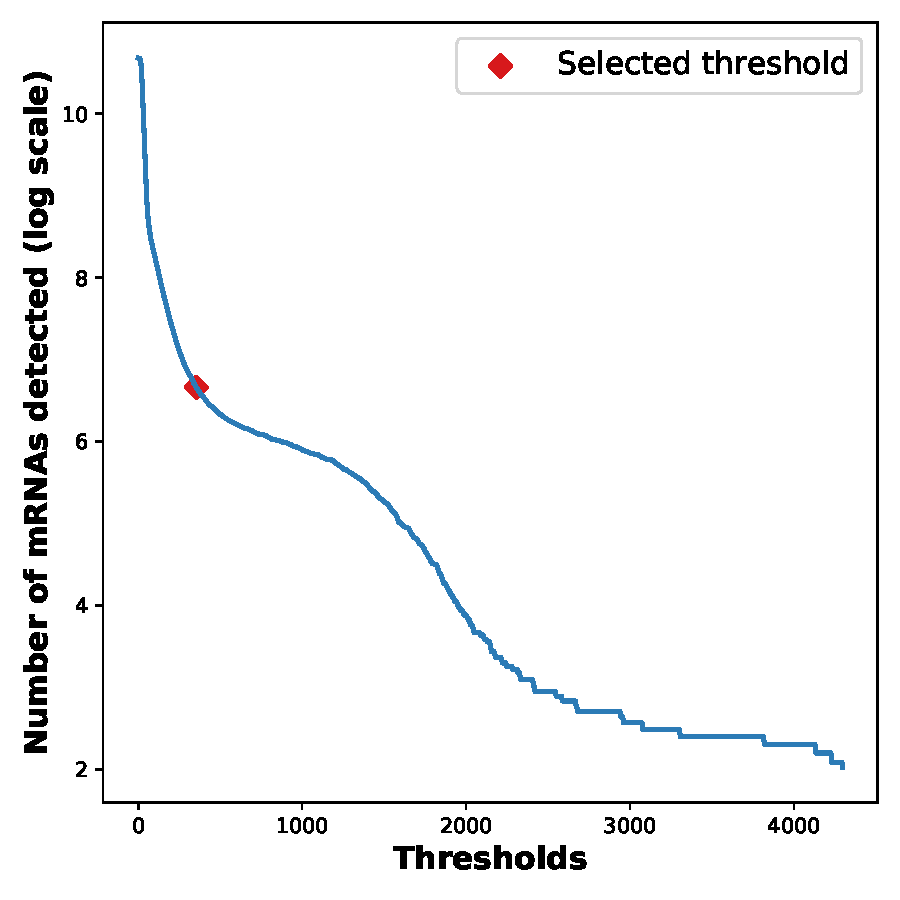
\includegraphics[width=0.33\textwidth]{figures/chapter2/elbow_curve_real}
	\caption{Elbow curve}
	\label{fig:elbow_detection}
	\end{center}
\end{wrapfigure}

We assume that a \ac{mRNA} spot and a background fluorescent noise have different intensity distribution.
The former have significantly higher intensity values since a \ac{mRNA} molecule is targeted by multiple oligos.
In the Figure~\ref{fig:elbow_detection}, we plot the relation between different thresholds and the number of remaining spots (with a log scale).
We observe a sharp and monotone decrease in the number of detected spots as we start increasing the detection threshold.
The \emph{spots} removed are mostly background noise at these low threshold levels.
Actual spots are too bright to be filtered out.
At the opposite, if we increase the threshold too much, we start removing real spots and the sensitivity of the detection decreases.
For a good image quality, the adequate intensity threshold corresponds to a plateau in the elbow curve~\ref{fig:elbow_detection}.
Even if this plateau is less pronounced with a high level of noise, an abrupt change in the slope of the curve is identifiable.
This difference of slope describes a clear separation between the regimes of overdetection and underdetection.

In order to automatically set an optimal threshold, we geometrically find the plateau of the elbow curve in~\ref{fig:elbow_detection}.
We select the threshold where the tangent's slope equals the average slope of the curve.
Additional elbow curves can be observed in appendix~\ref{sec:appendix_detection}, with different conditioning.\\

\begin{minipage}{0.9\textwidth}
\begin{lstlisting}[language=Python]
import bigfish.detection as detection

# spot detection with automated thresholding
spots, threshold = detection.detect_spots(
    images=smfish,
    return_threshold=True,
    voxel_size=(300, 103, 103),  # in nanometer
    spot_radius=(350, 150, 150))  # in nanometer
\end{lstlisting}
\end{minipage}

\subsection{Managing high spot density}
\label{subsec:dense_decomposition}

A second limitation in spot detection is to cope with clustered spots and high density areas, like active transcription sites or \ac{RNA} foci.
The method described above in~\ref{subsec:spot_detection} works well with isolated spots.
When spots are agglomerated, their shapes can't be resolved.
In addition, detection methods based on quick and sharp changes it term of pixel intensity might fails to detect a spot in a bright and uniform region.
In practice, an accumulation of spots looks like a large and bright fluorescent region where our detection will underestimate the number of individual spots.

Using a different (and larger) scale, a blob detection algorithm~\cite{walt_scikit-image_2014} might help to detect the cluster as a bigger spot.
However such method does not allow to decompose the cluster in individual spots.
In \emph{bigfish.detection} we adapt the solution proposed in MATLAB FISH-quant~\cite{mueller_fish-quant_2013}.
The latter detect the potential clusters and decompose them at the same time.
In the former we handle high spot density regions in two independent steps:

\begin{itemize}
	\setlength\itemsep{0.1em}
	\item We identify potential dense regions, then we decompose them in individual spots (mostly re-using the method from the first FISH-quant version).
	This step increases the number of detected spots in the image (see figure~\ref{fig:dense_decomposition}).
	\item We detect cluster of \ac{RNA}s by applying a clustering algorithm to the \ac{RNA} point cloud.
	This step can be performed with or without the dense region decomposition.
\end{itemize}

\subsubsection{Dense region detection}

\begin{wrapfigure}{R}{0.35\textwidth}
	\begin{center}
		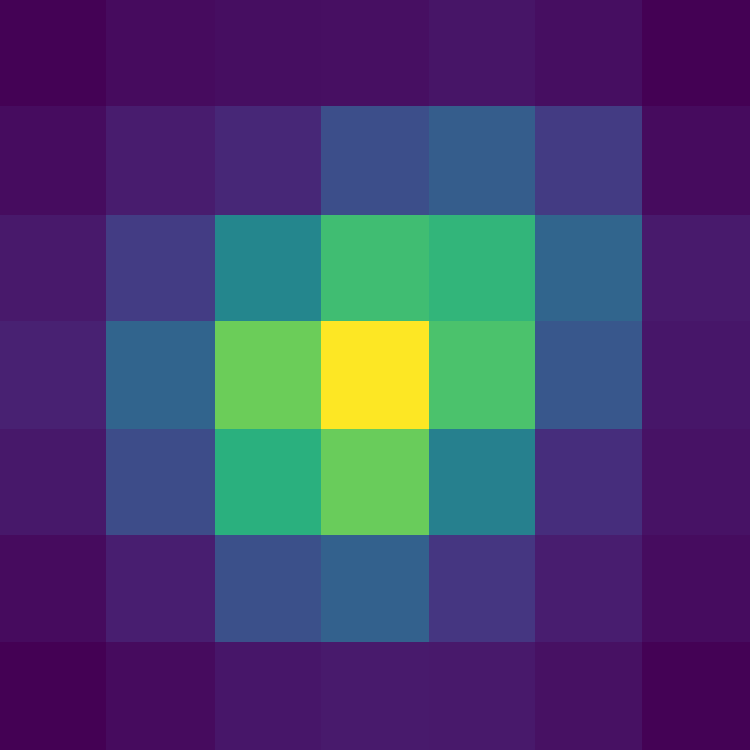
\includegraphics[width=0.33\textwidth]{figures/chapter2/reference_spot}
	\caption{Reference spot}
	\label{fig:reference_spot}
	\end{center}
\end{wrapfigure}

First step consists in localizing regions in the image with a probable cluster of spots.
We know that for such regions our detection might miss several spots.

We remove the low-frequency noise from the image by subtracting its background intensity.
The latter is approximated with a large Gaussian filtering.
From this denoised image we then extract the detected spots and compute the median spot signal.
This median signal is used as a threshold to filter the candidate regions with potential clustered spots.
We expect these regions to be brighter than individual spots, so they should at least be brighter than the median spot intensity.

A second criterion is the size of the regions.
They should be larger than an individual spot.
To match these criteria, we first threshold the denoised image with the median spot intensity, then we apply a connected component algorithm~\cite{wu_connected_component_2005} to the binary mask obtained.
Each group of connected pixels represent a region.
Because the mask is the result of a thresholding above the median spot signal, every region (or connected component) with at least 2 pixels are larger and brighter than the individual median spot.

\subsubsection{Dense region decomposition}

So far, the candidates regions can be actual clusters or simply an individual spot, brighter than the average.
We reuse the denoised image and aggregate the detected spots to compute a reference spot like in Figure~\ref{fig:reference_spot}.
By default this reference is the median spot, but another percentile can be chosen.
We fit a Gaussian signal on the reference spot to modelize it.
Such fit can be used to simulate new spots.

The decomposition process consists in populating our candidate regions by simulating as many spots as possible until we match the pixel intensity we observe.
Starting with an empty image, we iteratively add a new simulated spot in the region until we minimize the residual sum of square (RSS):

\begin{equation}
	{\displaystyle \operatorname{RSS} = \sum _{x, y}(\hat{f}(x, y) - f(x, y))^{2}}
\end{equation}

\noindent
with $\hat{f}(x, y)$ the simulated image intensity and $f(x, y)$ the denoised one.

\begin{figure}[h]
    \centering
    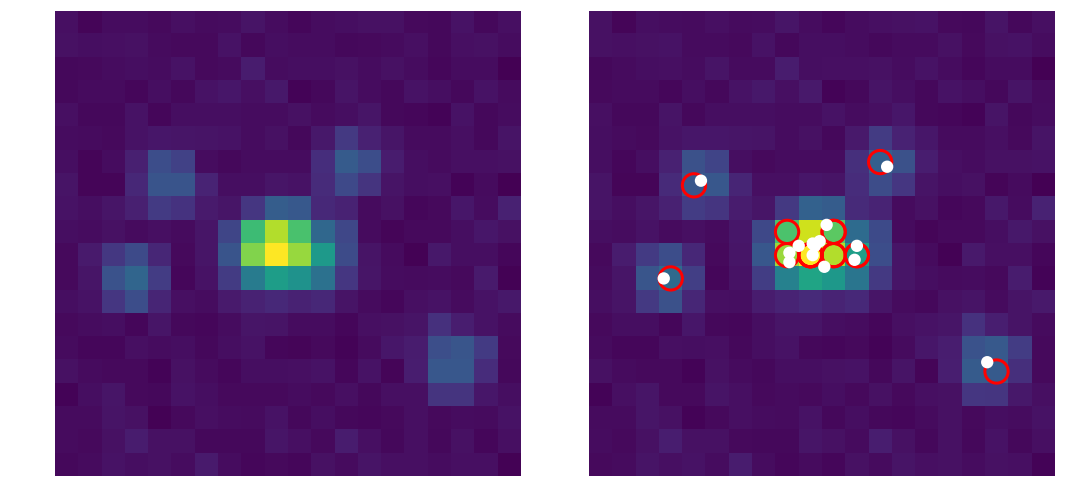
\includegraphics[width=1\textwidth]{figures/chapter2/plot_dense_decomposition}
    \caption{Decomposition results.
	(\textit{Left}) Original smFISH image zoomed in a dense region.
	(\textit{Right}) Detected spots in \textit{red} and actual clustered spots in \textit{white}}
    \label{fig:dense_decomposition}
\end{figure}

\subsubsection{Cluster detection}

The second independent step is the clustering itself.
Once we detect a \ac{RNA} point cloud, with or without the decomposition step, we look for \ac{RNA} clusters.

To this end we use a DBSCAN algorithm~\cite{ester_density-based_1996, scikit-learn}.
Two parameters need to be set: a minimum number of spots $k$ and a threshold distance $d$.
Every pair of \ac{RNA}s closer than $d$ are connected.
If a \ac{RNA} is connected to at least $k$ neighbors \ac{RNA}, it's a \emph{core sample} and with its connections it defines a cluster.
Such method allows us to detect clusters as ''areas of high density separated by areas of low density''\footnote{\url{https://scikit-learn.org/stable/modules/clustering.html}}.

Different users might may have a different definition of what they expect to be a cluster, depending of their analysis.
For the rest of the manuscript and throughout our studies, we usually consider a minimum group of 4 or 5 \ac{RNA}s within a radius of 350nm.
These are the default parameters in \emph{bigfish.detection} and the ones we use in Figure~\ref{fig:detection_results}.\\

\begin{minipage}{0.9\textwidth}
\begin{lstlisting}[language=Python]
import bigfish.detection as detection

# dense decomposition
spots_post_decomposition, _, _ = detection.decompose_dense(
    image=smfish,
    spots=spots,
    voxel_size=(300, 103, 103),  # in nanometer
    spot_radius=(350, 150, 150))  # in nanometer

# cluster detection
spots_post_clustering, clusters = detection.detect_clusters(
    spots=spots_post_decomposition,
    voxel_size=(300, 103, 103),  # in nanometer
    radius=350,  # in nanometer
    nb_min_spots=4)
\end{lstlisting}
\end{minipage}

\subsection{Going beyond pixel accuracy}
\label{subsec:subpixel}

Two additional methods already present in the first version of FISH-quant~\cite{mueller_fish-quant_2013} have been implemented in \emph{bigfish} as it is.

\subsubsection{Subpixel fitting}

So far, the spot detection and the dense region decomposition and the cluster detection return coordinates at the pixel level.
This can lead to a small inaccuracy, irrelevant for our own studies, but potentially critical for some users.
Such error can be observed in the Figure~\ref{fig:dense_decomposition} between the detected spots (with a pixel accuracy) and the ground truth (with a subpixel accuracy).

The possibility to refine the coordinate on individual spots solves this limitation.
We simply loop over the detected spots, crop their image and fit a gaussian signal on each of them.
We then correct the spot coordinates with the coordinates of the fitted gaussian.
Obviously, such method might return negative results in high density areas when spots can't be resolved.\\

\begin{minipage}{0.9\textwidth}
\begin{lstlisting}[language=Python]
import bigfish.detection as detection

# subpixel fitting
spots_subpixel = detection.fit_subpixel(
    image=smfish,
    spots=spots,
    voxel_size=(300, 103, 103),  # in nanometer
    spot_radius=(350, 150, 150))  # in nanometer
\end{lstlisting}
\end{minipage}

\subsubsection{Spot colocalization}

\begin{wrapfigure}{R}{0.35\textwidth}
	\begin{center}
		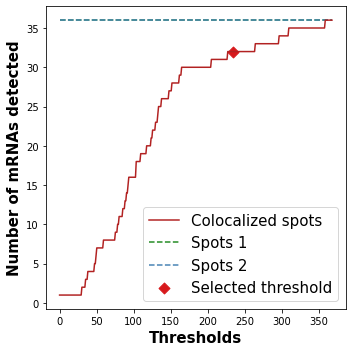
\includegraphics[width=0.33\textwidth]{figures/chapter2/colocalization_elbow}
	\caption{Threshold impact on colocalization}
	\label{fig:elbow_colocalization}
	\end{center}
\end{wrapfigure}

Another method requested by the community is the possibility to detect adjacent spots in different channels then match their coordinates.
Our implementation is based on the one developed in the recent work from~\cite{CORNES_2022}.
This could be the same \ac{RNA} detected with two different fluorescent probes or techniques.
As an example, in the Figure~\ref{fig:elbow_colocalization}, we detect colocalized spots between a sample of spots detected with a pixel accuracy and the same sample with a subpixel accuracy.

First we compute the euclidean distance matrix between the two sets of spot coordinates, then we solve a linear sum assignment problem~\cite{crouse_linear_assignment_2016, 2020SciPy-NMeth}.
We obtain an matching between the two sets of spots, for each spots, that minimize the overall euclidean distance between assigned pairs.
Finally, we only keep pairs with a distance below a specific threshold.
The Figure~\ref{fig:elbow_colocalization} illustrates the impact of the threshold parameter on the number of colocalized spots.
Like for the spot detection, we implement our heuristic~\ref{subsec:spot_detection} to infer an optimal threshold if none is provided.\\

\begin{minipage}{0.9\textwidth}
\begin{lstlisting}[language=Python]
import bigfish.multistack as multistack

# spot colocalization
(spots_1_colocalized, spots_2_colocalized,
 distances) = multistack.detect_spots_colocalization(
	spots_1=spots_crop,
	spots_2=spots_subpixel_crop,
	voxel_size=(300, 103, 103))  # in nanometer
\end{lstlisting}
\end{minipage}

% \cite{lagache_statistical_2015}
% Colocalization methods are traditionally divided into pixel-based methods
% that measure global correlation coefficients from the overlap between pixel
% intensities in different color channels, and object-based methods that first
% segment molecule spots and then analyze their spatial distributions with
% second-order statistics.

\section{Evaluation with simulated spots}
\label{sec:detection_evaluation}

Finally we describe our evaluation of \emph{bigfish.detection}.
In addition to qualitative assessment of spot detection throughout our studies, we quantify the accuracy errors with simulated images.
Performances for both spot and cluster detections are measured with different qualities of images.

\subsection{Simulations}
\label{subsec:simulation}

To measure the error of a spot detection we need a ground truth.
A manual annotation of a regular 3D \ac{smFISH} image is intractable.
It would be time-consuming and prone to human error.
The alternative is to simulate realistic images of spots, under different conditions to stress the performances of our algorithms.
To this end, we use the \emph{simfish} package that allows us to precisely control the level of noise and the number of spots we want to simulate in the image.

\subsubsection{Spot simulation}

The simulation process aims to return both an image and the ground truth coordinates of the spots we simulated.

\noindent
Our images are generated with three main steps:

\begin{enumerate}
	\item We randomly draw the number of spots and their localization.
	This is our ground truth.
	The number of spots is sampled from a Poisson distribution and the localizations from an Uniform distribution all over the frame.
	Alternatively the number of spots can be set manually.
	\item For each spot in the image we simulate its pixel intensity.
	Instead of directly sample the intensity value from a Gaussian distribution, we reuse the simulation process from~\cite{bahry_rs-fish_2021}.
	With a Gaussian distribution centered on every spot, we simulate the average number of photon collected by each pixel in the image.
	The amplitude and the standard deviation of this Gaussian signals are manually or randomly predetermined.
	The final intensity of every pixel is then sampled from a Poisson distribution with the number of photons as expectation.
	\item (Optional) We add a background white noise to the entire image.
	It follows a Normal distribution centered around a predefined noise level.
\end{enumerate}

% add a schema of the cluster simulation process if necessary

The process detailed above generate spots with a pixel accuracy.
A simulation with a subpixel accuracy follows the same steps, but with a larger image (4 to 20 times larger).
Before saving the image and the ground truth, we downsize it by local averaging.
The ground truth coordinates are adapted accordingly.

In order to produce a noisier image we can decrease the ratio between the spot amplitudes and the background noise.
A second option is to increase the variance of the different parameters: spot standard deviation and amplitude, background noise standard deviations.

\subsubsection{\ac{SNR}}

We can tune the different parameters mentioned to simulate spots with an increasing level of difficulty to detect.
To quantify the noise of an image and graduate the challenge it offers in term of detection, we compute its \ac{SNR} for every spot.

\noindent
For a 2D image, we define the $\operatorname{SNR}$ of an image as the median of the $\operatorname{SNR_i}$ we compute for each spot $i$, such that:

\begin{equation}
	{\displaystyle \operatorname{SNR_i} = \frac{\max(a(x, y)) - \mu(b(x, y))}{\sigma(b(x, y))}}
\end{equation}

\noindent
with $\mu(.)$ the mean function, $\sigma(.)$ the standard deviation, $a(x, y)$ the spot image cropped and $b(x, y)$ the spot background (a crop twice larger than the spot image).

In consequence, our measure of noise is based on the spot coordinates.
We quantify how distinct the spot is from its background.
A spot with a low amplitude or a noisy background will decrease the \ac{SNR} of the image.
To correctly quantify the image noise during our evaluation, we use the ground truth coordinates of the spots to compute the \ac{SNR}.
Indeed, a noisy image would impact the detection and bias the measure of noise itself.
We simulate different images with a range of \ac{SNR} between 2 and 26.
The higher the \ac{SNR} is, the better.

For example, in Figure~\ref{fig:spot_detection_high_noise} we simulate an extreme case with a highly noisy image (\ac{SNR} below 5).
On the right panel we can observe some contrasted background blobs misdetected as spot.
Despite a small amount of false positives, the detection remains correct in this badly conditioned image.

\begin{figure}[h]
    \centering
    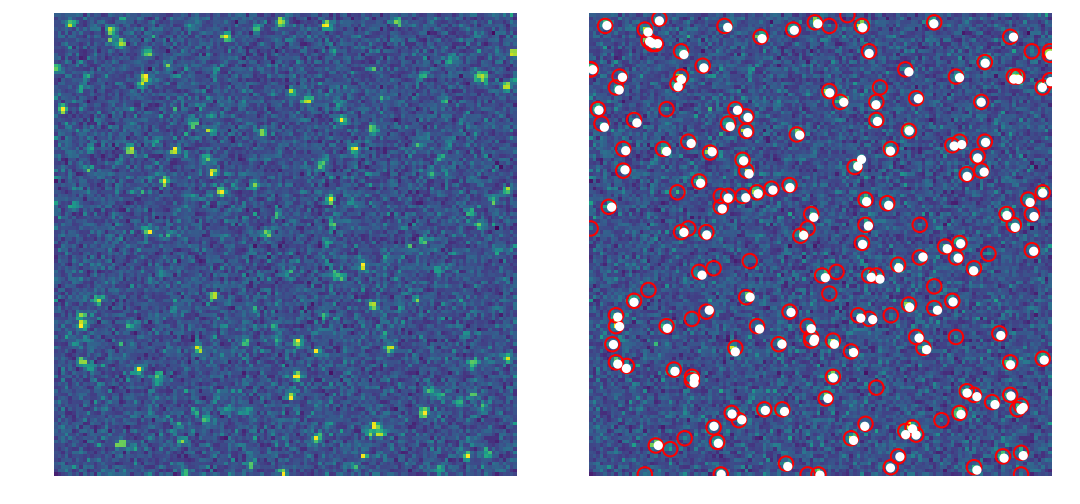
\includegraphics[width=1\textwidth]{figures/chapter2/plot_spot_detection}
    \caption{Noisy spot simulation with \emph{simfish}.
	(\textit{Left}) Original simulated image.
	(\textit{Right}) Detected spots in \textit{red} and actual spots in \textit{white}}
    \label{fig:spot_detection_high_noise}
\end{figure}

\subsubsection{Cluster simulation}

The user can also decide to simulate clusters.
In this case, the first step of our simulation process is adapted.
First the number of clusters and the number of spots per cluster are drawn from a Poisson distribution (or manually set).
The cluster centers are then localized like spots, with a Uniform distribution over the entire image, or fixed at the center of the frame.
Finally, different spot localizations are randomly generated around the centers, using polar coordinates.
The result can be observed in Figure~\ref{fig:dense_decomposition} which is actually a simulated cluster.
In addition, several simulations are available in appendix~\ref{sec:appendix_simulations_spots}, with different conditioning.\\

\begin{minipage}{0.9\textwidth}
\begin{lstlisting}[language=Python]
import simfish as sim

# image simulation
image, ground_truth = sim.simulate_image(
	ndim=3,
	n_spots=100,
	image_shape=(128, 128),
	voxel_size=(100, 100, 100),  # in nanometer
	sigma=(150, 150, 150),  # in nanometer
	amplitude=5000,
	noise_level=300)
\end{lstlisting}
\end{minipage}

\subsection{Results}
\label{subsec:detection_results}

We simulated batches of 100 images with high, medium and low noise levels (roughly, with a \ac{SNR} below 5, between 5 and 15 and above 15).

\subsubsection{Impact of noise}

Our method is overall pretty robust.
If the image quality deteriorates, with a lower \ac{SNR} for example, our algorithms can return a moderate overestimation of detected spots.
This overestimation is estimated below 5\% and 10\% for images with a low or medium \ac{SNR} value, respectively.

These measures are illustrated on the left panel of Figure~\ref{fig:detection_error}.
We compared the number of spots detected with the actual number of spots simulated.
Each dot corresponds to one image.
For each noise regime, 100 images are generated.
Above the plain line, the detection overestimates the number of spots.
Logically, these overestimations increase with the noise level (and decrease with the \ac{SNR}).

On the right panel, we summarize the impact of noise with our detection technique.
Each dot represents again an image, with 100 simulated spots and a varying level of noise.
Below a \ac{SNR} of 5, with poorly contrasted spots, a fully automated detection might remain challenging.

\begin{figure}[h]
    \centering
    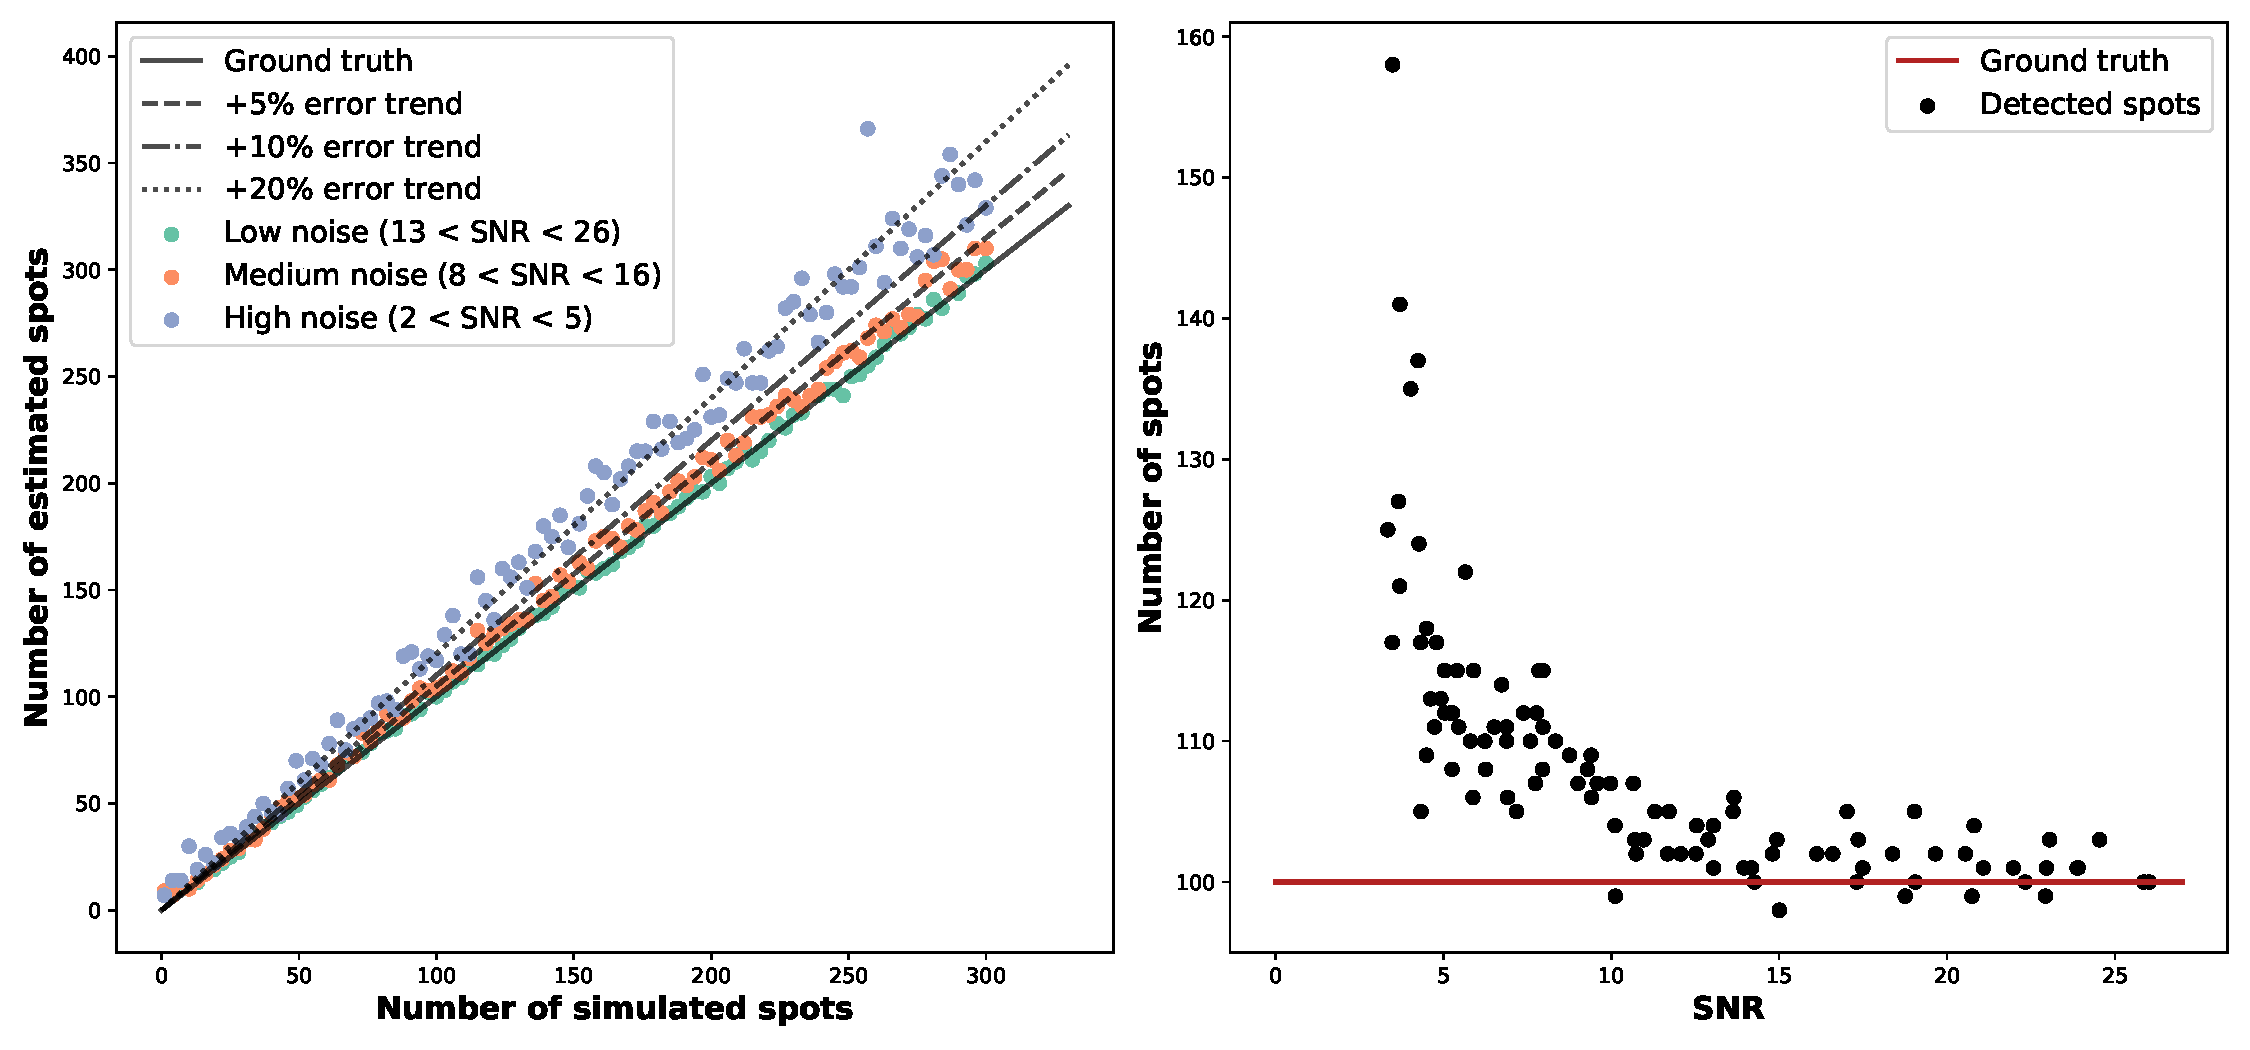
\includegraphics[width=1\textwidth]{figures/chapter2/fused_spot_detection_noise}
    \caption{Impact of noise on automated detection.
	(\textit{Left}) Number of detected spots for different numbers of simulated spots.
	(\textit{Right}) Number of detected spots for different levels of noise (with 100 simulated spots)}
    \label{fig:detection_error}
\end{figure}

\subsubsection{Accuracy of the cluster detection}

We simulate images with a unique cluster in order to test the performance of our method to decompose the dense regions and detect the clusters.
Such images can be observed in appendix~\ref{sec:appendix_simulations_spots}.
In Figure~\ref{fig:cluster_results} we report the number of spots we estimate in the clusters.
Each dot represent an image with a cluster.
Our decomposition is quite robust with the noise level, even with the lower \ac{SNR} values.
However, for the largest clusters, with 15 spots or more, we tend to slightly underestimate the number of spots.
In this case, the average error is 1.6.
In comparison, with 5 spots and 10 spots per cluster, we measure an average error of 0.83 and 0.82, respectively.

\begin{figure}[h]
    \centering
    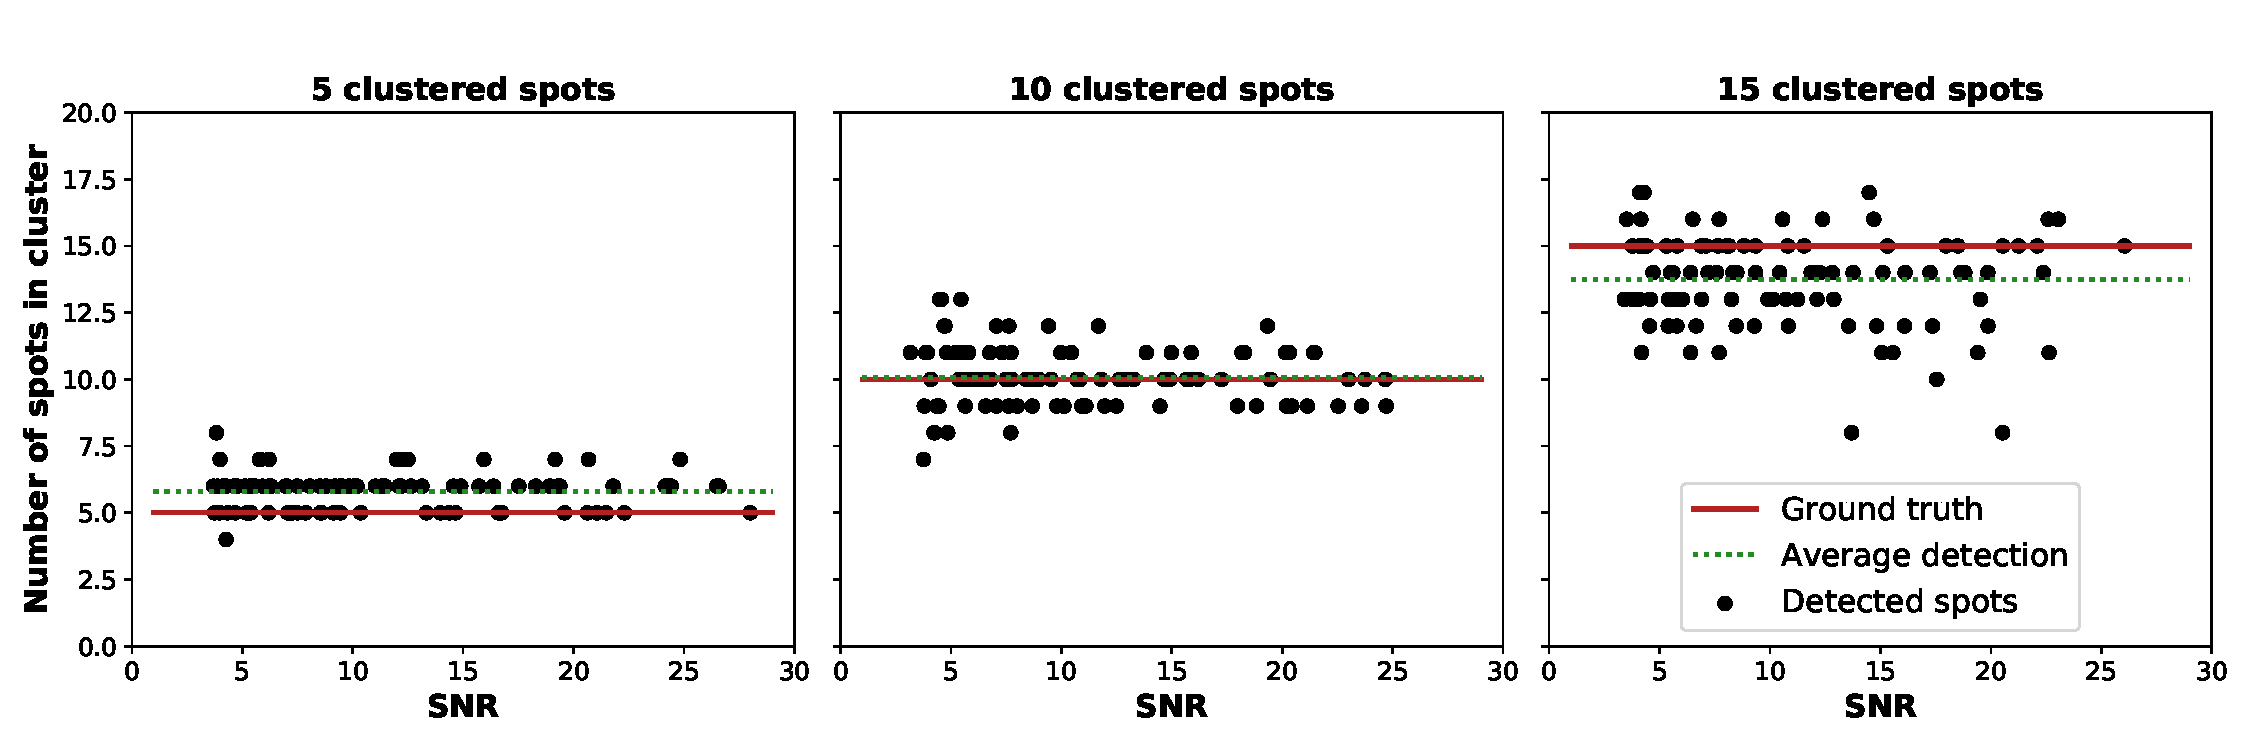
\includegraphics[width=1\textwidth]{figures/chapter2/cluster_along_noise}
    \caption{Dense region decomposition evaluation.
	 Number of spots estimated per cluster for different levels of noise and respectively 5 (\textit{left}), 10 (\textit{center}) or 15 (\textit{right}) simulated spots per cluster}
    \label{fig:cluster_results}
\end{figure}

\subsection{What if the \ac{PSF} is not Gaussian?}
\label{subsec:psf}

In this chapter we assume our \ac{mRNA} spots can be modelled with a Gaussian signal.
This simplification was relevant during my PhD and did not lead to exaggerated errors in our different analysis.
However, it is always possible to exploit a more complex \ac{PSF} to fit with a specific spot signal.
To this end, the former \emph{psf} package\footnote{\url{https://github.com/cgohlke/psf/}} allows to generate more complex \ac{PSF} for specific fluorescent microscopic experiments.
Letting the user choose between different \ac{PSF} is an improvement that could be implemented in in a future version of \emph{bigfish.detection} and \emph{simfish}.
In particular, this would modify the way we generate spot signal in our image simulations or in the decomposition of dense regions.

Eventually, if the \ac{PSF} differs greatly from a Gaussian signal, the spot detection itself could be impacted.
Indeed, two \ac{PSF}s from close spots could interfere and make the local peaks less distinct.

% potential references in PSF
% Electromagnetic diffraction in optical systems. II. Structure of the image field in an aplanatic system. B Richards and E Wolf. Proc R Soc Lond A, 253 (1274), 358-379, 1959.
% Focal volume optics and experimental artifacts in confocal fluorescence correlation spectroscopy. S T Hess, W W Webb. Biophys J (83) 2300-17, 2002.
% Electromagnetic description of image formation in confocal fluorescence microscopy. T D Viser, S H Wiersma. J Opt Soc Am A (11) 599-608, 1994.
% Photon counting histogram: one-photon excitation. B Huang, T D Perroud, R N Zare. Chem Phys Chem (5), 1523-31, 2004. Supporting information: Calculation of the observation volume profile.
% Gaussian approximations of fluorescence microscope point-spread function models. B Zhang, J Zerubia, J C Olivo-Marin. Appl. Optics (46) 1819-29, 2007.
% The SVI-wiki on 3D microscopy, deconvolution, visualization and analysis. https://svi.nl/NyquistRate
% Theory of Confocal Microscopy: Resolution and Contrast in Confocal Microscopy. http://www.olympusfluoview.com/theory/resolutionintro.html

\section{Conclusion}
\label{sec:detection_conclusion}

This chapter presents different methods from \emph{bigfish.detection} subpackage to perform a spot detection on \ac{FISH} images.
Based on the first version of FISH-quant, the main contribution of these algorithms are their ability to detect spots without tuning any pixel intensity threshold.
We evaluate the performance on simulated images and find the detection robust enough to be applied on a high content screening experiment.
Our method currently overcomes human intervention and makes the processing of thousands different images possible.

Of course, several improvements are still possible.
We can expand the \ac{PSF} options as explained in~\ref{subsec:psf}.
Some alternative detection techniques claim a better accuracy or faster runs like~\cite{bahry_rs-fish_2021}.
A Python implementation of these methods, coupled with our thresholding heuristic to scale the detection, might be valuable for the community.

% https://github.com/PreibischLab/RS-FISH/tree/master/documents/tool_comparison_for_paper